% Q5V1: GPR through soil — Signal path diagram
% Physical setup: antenna on surface → soil → buried pipe → soil → air → Rx
% No formulas in diagram (P-STACK-31: given in question text)
\documentclass[border=10pt]{standalone}
\usepackage{tikz}
\usepackage{amsmath}
\usetikzlibrary{arrows.meta, decorations.pathreplacing}
\renewcommand{\familydefault}{\sfdefault}

\begin{document}
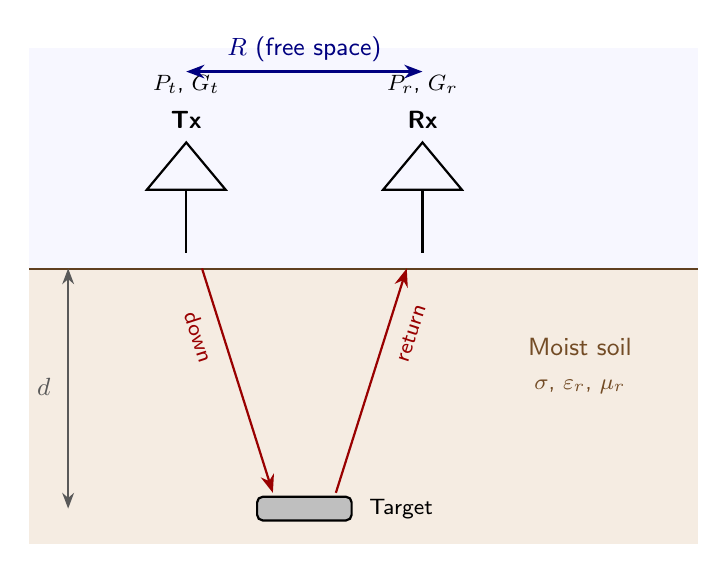
\begin{tikzpicture}[
    every node/.style={font=\sffamily},
    >=Stealth,
]

% === Ground surface ===
\fill[brown!15] (-0.5,-3.5) rectangle (8,0);
\draw[thick, brown!50!black] (-0.5,0) -- (8,0);
\node[above left, font=\sffamily\footnotesize, brown!50!black] at (8,0.05) {Ground surface};

% === Air region ===
\fill[blue!3] (-0.5,0) rectangle (8,2.8);

% === GPR Tx/Rx unit (on surface) ===
% Tx antenna
\draw[thick] (1.5, 0.2) -- (1.5, 1.0);
\draw[thick] (1.0, 1.0) -- (1.5, 1.6) -- (2.0, 1.0) -- cycle;
\node[above, font=\sffamily\small\bfseries] at (1.5, 1.65) {Tx};
\node[above, font=\sffamily\footnotesize] at (1.5, 2.1) {$P_t$, $G_t$};

% Rx antenna
\draw[thick] (4.5, 0.2) -- (4.5, 1.0);
\draw[thick] (4.0, 1.0) -- (4.5, 1.6) -- (5.0, 1.0) -- cycle;
\node[above, font=\sffamily\small\bfseries] at (4.5, 1.65) {Rx};
\node[above, font=\sffamily\footnotesize] at (4.5, 2.1) {$P_r$, $G_r$};

% === Buried pipe (reflection target) ===
\fill[gray!50, draw=black, line width=0.8pt, rounded corners=2pt]
    (2.4,-2.9) rectangle (3.6,-3.2);
\node[right, font=\sffamily\footnotesize] at (3.7, -3.05) {Target};

% === Signal path arrows ===
% Down path (Tx → pipe)
\draw[->, thick, red!60!black] (1.7, 0) -- (2.6, -2.85);
\node[left, font=\sffamily\footnotesize, red!60!black, rotate=-72] at (1.8, -1.3) {down};
% Up path (pipe → surface)
\draw[->, thick, red!60!black] (3.4, -2.85) -- (4.3, 0);
\node[right, font=\sffamily\footnotesize, red!60!black, rotate=72] at (4.2, -1.3) {return};

% === Air path (surface to Rx) ===
\draw[<->, thick, blue!50!black] (1.5, 2.5) -- (4.5, 2.5);
\node[above, font=\sffamily\small, blue!50!black] at (3, 2.5) {$R$ (free space)};

% === Soil medium labels ===
\node[font=\sffamily\small, brown!60!black] at (6.5, -1.0) {Moist soil};
\node[font=\sffamily\footnotesize, brown!60!black] at (6.5, -1.5) {$\sigma$, $\varepsilon_r$, $\mu_r$};

% === Dimension: soil depth ===
\draw[<->, line width=0.6pt, gray!70!black] (0, 0) -- (0, -3.05);
\node[left, font=\sffamily\small, gray!70!black] at (-0.1, -1.5) {$d$};

\end{tikzpicture}
\end{document}
